\documentclass[10pt, a4paper]{article}
\usepackage{lrec2006}
\usepackage{graphicx}

\usepackage[utf8]{inputenc}

\usepackage{hyperref}
\usepackage{alltt}
\usepackage{amsmath}

\title{Attaching Translations to Proper Lexical Senses in DBnary}

\name{Andon Tchechmedjiev, Gilles Sérasset, J\'{e}r\^{o}me Goulian, Didier Schwab }

\address{ LIG-GETALP, Univ Grenoble Alpes\\
               BP 53 – 38051 Grenoble cedex 9 \\
               \texttt{firstname.lastname@imag.fr}\\}


\abstract{ 
The DBnary project aims at providing high quality Lexical Linked Data extracted from different Wiktionary language editions. Data from 10 different languages is  currently extracted for a total of over $3.16$M translation links that connect lexical entries from the 10 extracted languages, to entries in more than one thousand languages. 
In Wiktionary, glosses are often associated with translations to help users understand to what sense they refer to, wether through a textual definition or a target sense number. In this article we aim at the extraction of as much of this information as possible and then the disambiguation of the corresponding translations for all languages available. We use an adaptation of various textual and semantic similarity techniques based on partial or fuzzy gloss overlaps to disambiguate the translation relations (to account for the lack of normalization, e.g. lemmatization and PoS tagging) and then extract some of the sense number information present to build a gold standard so as to evaluate our disambiguation as well as tune and optimize the parameters of the similarity measures.
We obtain F1 score of the order of 80\% (on par with similar work on English only), across the three languages where we could generate a gold standard (French, Portuguese, Finnish) and show that most of the disambiguation errors are due to inconsistencies in Wiktionary itself that cannot be detected during the generation of DBnary (shifted sense numbers, inconsistent glosses, etc.). \\ \newline \Keywords{Wiktionary, Linked Open Data, Multilingual Resources}}


\DeclareMathOperator*{\argmax}{arg\!\max}
%\DeclareMathOperator*{\max}{\max}
\begin{document}

\maketitleabstract

\section{Introduction}

Wiktionary is a lexical-semantic resource built collaboratively under the patronage of the Wikimedia Foundation (which also hosts the well known Wikipedia initiative). It is currently the biggest collaborative resource for lexical data. Wiktionary pages usually describe lexical entries by giving their part of speech, a set of definitions, examples, lexico-semantic relations and many translations in more than a thousand target languages.

The DBnary project \cite{serasset:dbnary-swj} aims at providing high quality Lexical Linked Data extracted from different Wiktionary language editions. It currently extracts data from 10 editions and gathers $3.16$M translation links relating lexical entries from the 10 extracted languages to entries in more than a thousand languages. These numbers are steadily growing as the DBnary dataset is extracted as soon as Wikimedia releases new dumps of the data (around once every 10-15 days for each language edition).

The sources of these translation links are \emph{lexical entries}. The purpose of this work is to attach these translations to the correct \emph{word sense} and hence to increase the value and quality of the DBnary dataset. Comparable efforts have been carried out (mainly on the UBY dataset), but are limited to English and German. In this paper we worked on 10 language editions. Among them, we were faced with the various habits of the different Wiktionary communities. For example different languages editions exhibit different linguistic properties. 
After detailing related works, we present the structure of the DBnary dataset. Then, after showing how we built an endogenous golden standard used to evaluate this work, we detail the methods used to achieve our purpose. Finally we evaluate our method and discuss the results.

\section{Related Work}

\subsection{Extracting Data from Wiktionary Language Editions.} Since its inception in 2002, Wiktionary has steadily increased in size (both with collaborative work and with automatic insertions of available lexical data). Interest in Wiktionary as a source for lexical data for NLP applications has quickly risen. Studies like \cite{Zesch:AAAI2008} or \cite{navarro-EtAl:2009:PeoplesWeb} show the richness and power of this resource. 

Since then, efforts have mostly been focussed on the systematic extraction of Wiktionary data. Many of them, as resources for a specific project and thus merely snapshots of Wiktionary at a fixed point in time. As all Wiktionary language editions evolve regularly (and independently) in the way their data is represented, such efforts are not suitable to provide a sustainable access to Wiktionary data. 

Some efforts, however are maintained and allow access over time. One of the most mature project is the \emph{JWKTL} API \cite{ZeschMuellerGurevych2008} giving access to  the English, German and Russian language editions. It is used in the UBY project \cite{gurevych2012uby} which provides an LMF based version of these editions. 

We should also mention the wikokit project \cite{krizhanovsky2010transformation} that provides access to the English and Russian editions and that was used by \emph{JWKTL}.

\cite{HellmannSebastianandBrekleJonasandAuer} presents another attempt under the umbrella of the DBpedia project \cite{dbpedia-swj}, whose purpose is specifically to provide the Wiktionary data as Lexical Linked Open Data. The main reason this approach is interesting is the collaborative nature extraction template creation process (following the culture of the DBpedia project). Currently English, French, Russian and German Wiktionary editions are supported.

This paper is part of the DBnary project \cite{serasset:dbnary-swj} that has a similar purpose to that of \cite{HellmannSebastianandBrekleJonasandAuer}. Our goal is to provide LEMON \cite{McCrae2012} based lexical databases that are structured like traditional lexica. Indeed, we extract data from Wiktionary, but we currently restrict ourselves to the ``native'' data of each language edition, e.g. the French data is extracted from the French language edition and we disregard French data contained in other editions. To the best of our knowledge DBnary is currently the most advanced extractor for Wiktionary with an active support of 10 languages. It is also the only initiative giving access to the whole extracted data history.

\subsection{Disambiguation of the Source of Translations.} 

As far as attaching translations to the proper word sense (translation disambiguation) is concerned, the most similar work to ours is that of \cite{meyer-gurevych:2012:PAPERS}. Their intent matches our own, however their efforts only deal with the German and English editions. In their work, the gold standard was manually created and was significantly smaller than the endogenous gold standard we extracted from the resource itself. They use a backoff strategy (to the most frequent sense) when the heuristic based on similarity measures and the resource's structure fails. The other heuristics used with their similarity measure also imply a finer analysis of definitions and glosses so as to distinguish between linguistic labels (domain, register, title, etc.).

Herein, we achieve similar scores on the languages we were able to evaluate with an endogenous gold standard, even though we only used string and token similarity measures in the context of languages with less common features (e.g. the agglutinative aspect of the Finnish language).

\subsection{Similarity measures}
Our method is based on the application of gloss overlap measures and their extension with ideas taken from Hybrid textual similarity measures that match sentences both at the character and at the token level. In the work mentioned above \cite{meyer-gurevych:2012:PAPERS}, a feature-based similarity is used (gloss overlap), while in some of their prior work \cite{MeyerGurevych:2010},  they use a textual similarity measure based on vector-spaces generated from corpora (Explicit Semantic Analysis).

We propose a simple similarity measure where we replace the exact word match of the overlap calculation with an approximate string distance measure and place ourselves in the general framework of the Tversky \cite{tversky77similarity} index (can be seen as a generalization of Lesk, the Dice coefficient , the Jaccard and Tatimono indexes, etc.)

The idea of ``soft-cardinality'' proposed by \cite{Jimenez2010,Jimenez2012} is very similar in the sense that it exploits the Tversky index as a base and conjugates it with a textual similarity measure. That is, instead of incrementing the overlap count by 0 or 1, incrementing it by the value returned by the text similarity measure between the current pair of words being considered in the overlap calculation.
 
Their text similarity measure is based on an an empirical q-gram model (character-grams that correspond to substrings) combined with point-wise mutual information weighting. However in our work, generating a language model for 10 languages would require considerable effort and with future additions of more languages, become a daunting task. 
  
In the textual similarity tasks in SemEval, using approximate string matching for overlap calculation is not new and has been exploited by several system, including in 2013 a soft cardinality system by \cite{Jimenez2013} or other systems such as that of \cite{Wu2013} who use longest common sub-strings and greedy string tiling .
 
As such, we chose to use a simple string distance measure for the approximate string match calculations. However, there are many such measure and it is necessary to select the right one for the task as will be detailed in Section \ref{sec:expe} Moreover, there are existing so called ``Level 2'' or ``Hybrid'' similarity measures that already combine token overlap with token distance measures. Thus, we will need to evaluate our proposed method with some of the existing methods so as to evaluate their viability. The various measures and a detailed performance comparison in a name matching task are presented by \cite{Cohen2003}.

\section{The DBnary Dataset}

DBnary is a Lexical Linked Open Dataset extracted from 10 Wiktionary language editions (English, Finnish, French, German, Greek, Italian, Japanese, Portuguese, Russian and Turkish). It is available on-line at \url{http://kaiko.getalp.org/about-dbnary}. DBnary currently contains 35+M triples. This number is steadily growing as the dataset evolves in parallel with the original Wiktionary data. Indeed, the dataset is automatically updated as soon as Wikimedia releases new Wiktionary dumps, i.e. every 10-15 days per language edition. 

DBnary is structured according the LEMON ontology for lexical linked data \cite{McCrae2012}. Table \ref{lemon-elts} shows the number of Lexical Elements, as defined in the LEMON ontologies, for the different extracted languages. 

The elements in DBnary that couldn't be represented with LEMON, were defined as a custom ontology built on top of existing LEMON classes and relations, most notably lexico-semantic relation and what we call \verb|Vocables|, the top level entries in Wiktionary that correspond to Wiktionary pages for specific words, and that can contain several \verb|lemon:LexicalEntry|s categorised in two levels:
\begin{enumerate}
	\item Homonymous distinction of words of different etymological origins (e.g. \verb|river [water stream]| v.s. \verb|river [one who rives or split])|
	\item For each etymological origin, the different lexico-grammatical categories (PoS) (e.g. \verb|cut#V| \verb|[I cut myself]| v.s. \verb|cut#Noun| \verb|[I want my cut of the winning]|)
\end{enumerate}


\begin{table*}[htb!]
\begin{center}\begin{footnotesize}
\begin{tabular}{lrrrrrrr}
\textbf{Language} & \textbf{Entries} & \textbf{LexicalSense} & \textbf{Translations} & \textbf{Glosses} & \textbf{Text} &  \textbf{Sense Num} & \textbf{Text+Sense Num.}\\
\hline
English & $544,338$ & $438,669$ & $1,317,545$ & $1,288,667$ & $1,288,667$ & $515$ & $515$ \\
Finnish & $49,620$ & $58,172$ & $121,278$ & $120,728$ & $120,329$ & $115,949$ & $115,550$ \\
French & $291,365$ & $379,224$ & $504,061$ & $136,319$ & $135,612$ & $28,821$ & $28,114$ \\
German & $205,977$ & $100,433$ & $388,630$ & $388,553$ & $3,101$ & $385,452$ & $0$ \\
Modern Greek & $242,349$ & $108,283$ & $56,638$ & $8,368$ & $8,368$ & $12$ & $12$ \\
Italian & $33,705$ & $47,102$ & $62,546$ & $0$ & $0$ & $0$ & $0$ \\
Japanese & $24,804$ & $28,763$ & $85,606$ & $22,322$ & $20,686$ & $4,148$ & $2,512$ \\
Portuguese & $45,109$ & $81,023$ & $267,048$ & $74,901$ & $72,339$ & $71,734$ & $69,172$ \\
Russian & $129,555$ & $106,374$ & $360,016$ & $151,100$ & $150,985$ & $115$ & $0$ \\
Turkish & $64,678$ & $91,071$ & $66,290$ & $53,348$ & $585$ & $52,901$ & $138$ \\
\hline
\end{tabular}
\caption{Number of elements in the current DBnary dataset, detailing the number of entries and word senses, along with the number of translations. The table also details the number of Glosses attach to translations, among which the amount of textual glosses, of glosses giving the sense identifier and, finally, the number of glosses that contain both a textual description and a word sense identifier.}
\label{lemon-elts}
\end{footnotesize}\end{center}
\end{table*}

\subsection{Translation relations}

The DBnary dataset represents translation relations in an ad-hoc manner: the LEMON model does not have a vocabulary for such information. A \verb|Translation| is a RDF resource that gathers all extracted information pertaining to a translation relation. For instance, one of the translations of the lexical entry \emph{frog} is represented as follows\footnote{The Turtle syntax is used throughout the paper for RDF data.}:

\begin{small}
\begin{alltt}
eng:__tr_fra_1_frog__Noun__1
      a       dbnary:Translation ;
      dbnary:gloss "amphibian"@en ;
      dbnary:isTranslationOf
              eng:frog__Noun__1 ;
      dbnary:targetLanguage
              lexvo:fra ;
      dbnary:usage "f" ;
      dbnary:writtenForm "grenouille"@fr .
\end{alltt}
\end{small}

The properties of this resource point to the source \verb|LexicalEntry|, the language of the target (represented as a \verb|lexvo.org| entity \cite{deMeloWeikum2008c}), the target written form and optionally, a gloss and usage notes.

Usage notes give information about the target of the translation (e.g. the gender or a transcription of the target).

The gloss gives disambiguation information about the source of the translation. In the example given, it states that the given translation is valid for the word sense of \emph{frog} that may be described by the hint ``\emph{amphibian}''. Some of these glosses are textual and summarize or reprise the definition or part thereof for one or more specific sense to which the translation specifically applies to.

As an example, the English \verb|LexicalEntry| \emph{frog} contains 8 word senses, defined as follows:

\begin{small}\begin{enumerate}
\item A small tailless amphibian of the order Anura that typically hops
\item The part of a violin bow (or that of other similar string instruments such as the viola, cello and contrabass) located at the end held by the player, to which the horsehair is attached
\item (Cockney rhyming slang) Road. Shorter, more common form of frog and toad
\item The depression in the upper face of a pressed or handmade clay brick
\item An organ on the bottom of a horse’s hoof that assists in the circulation of blood
\item The part of a railway switch or turnout where the running-rails cross (from the resemblance to the frog in a horse’s hoof)
\item An oblong cloak button, covered with netted thread, and fastening into a loop instead of a button hole.
\item The loop of the scabbard of a bayonet or sword. 
\end{enumerate}\end{small}

Translations of this entry are divided in 4 groups corresponding to: ``\emph{amphibian}'', ``\emph{end of a string instrument’s bow}'', ``\emph{organ in a horse’s foot}'' and ``\emph{part of a railway}''. 

Additionally among the glosses, some may contain sense numbers, indicated by users in an ad-hoc way (may or may not be present, and if they are no standard format is systematically followed or enforced). Furthermore, the presence of disambiguation information is very irregular and varies greatly between languages, both in terms of wiki structure and representation.

In the current state of the Wiktionary extraction process, we extract translation and when possible the associated glosses. However up to now, we have not exploited the information contained in the glosses to enrich and disambiguate the source senses of translation relations.

As mentioned above, the information contained in translation glosses and their format is very variable across languages, both quantitatively and qualitatively. 

Indeed, as shown in Table \ref{lemon-elts} some language like Italian, contain no gloss altogether, others, like English attaches textual glosses to translations almost systematically, but with no sense numbers. Others still, like German hardly contain textual glosses but give sense numbers to translations. In other cases, such as for Finnish, French and Portuguese, many translations have an attached (textual) gloss with associated sense numbers. 

In order to evaluate our method we use mixed glosses that both contain a textual hint and a sense number, so as to create a endogenous gold standard.

\subsubsection{Creation of a gold standard}

False positives and variability are often present among available translation glosses that do contain textual information or sense numbers due the variety of structures employed in Wiktionary as well as artefacts resulting from the extraction process. Before we can proceed further we need to filter this information so as to keep only the relevant parts. However, no other preprocessing is performed.

More concretely two steps must be followed if we are to successfully extract the information we need :
\begin{itemize}
   \item Remove empty glosses, or glosses containing irrelevant textual content that often correspond to TO DO notes in various forms (e.g. \emph{translations to be checked})
   \item Extract sense numbers from the glosses when available using language dependent templates (e.g. ``\emph{textual gloss (1)}'' or ``\emph{1. textual gloss}'') 
\end{itemize}

When enough glosses contained both a textual hint and sense numbers, we removed the sense numbers\footnote{Translation are ban be valid for several source senses} from the gloss and used them to create a gold standard in the trec\_eval format. Only three of the ten language met the requirements as for many of the 10 languages there are no numbered glosses or no translation glosses altogether.

After successfully extracting as much information as possible from translation glosses, we disambiguatthe translation. While, the steps above are indeed language specific, our process is designed to be as generic and computationally efficient as possible. Indeed, we are required to periodically perform the disambiguation, whenever a new version of DBnary is extracted from the latest Wiktionary dumps.

\section{Attaching Translations to Word Senses}
\subsection{Formalization of translation disambiguation}
Let \(T\) be the set of all translation relations, \(L\) the set of all \verb|LexicalEntry| in a given language edition of DBnary. Let \(T_i\in T: Gloss(T_i)\) be a function that returns the gloss of any translation \(T_i\in T\) and let \(Source(T_i)=L_{T_i}\) be a function that returns a reference to the source \verb|LexicalEntry|, \(L_{T_i}\) of a translation \(T_i\). Let \(Senses(L_i)=S_{L_i}\) be the set of all the senses associated with \verb|LexicalEntry| \(L_i\). Let \(S_{L_i}^k\) be the \(k\)-th sense contained in \(S_{L_i}\) and let \(Def(S_{L_i}^k)\) be a function that returns the textual definition of a sense \(S_{L_i}^k\). Finally let \(Sim(A,B)\) be a function that returns a semantic similarity or relatedness score between \(A\) and \(B\), where \(A,B\) are a pair of textual definitions or textual glosses. 

Then, we can express the disambiguation process as:
\[
\forall T_i \in T, S=Senses(Source(T_i)): 
\]
\[
Source^*(T_i) \leftarrow  \argmax_{S^k\in S} \{Score(Gloss(T_i),Def(S^k))\}
\]

This corresponds exactly to a standard semantic similarity maximisation and yields one disambiguated source sense per translation. However in many cases a translation corresponds to one or more senses. The solution adopted by \cite{MeyerGurevych:oup2012} is to use a threshold \(k\) for their gloss overlap, however in our case, we want to be able to plug-in several different measures so as to find the most suitable one, thus, fixed and arbitrary value for \(k\) is not an option. Thus, we need to add one more constraint: that the values returned by our similarity function need to be normalized between \(0 \mbox{ and  } 1\).

Here, instead of taking a threshold \(k\), we set a window \(\delta\) around the best score in which the senses are accepted as a disambiguation of a given translation. We hypothesise that a relative threshold dependant on the maximal score will set a precedent and be more representative of the possible range of values. Of course, setting a fixed threshold has the effect of not assigning any senses if all the scores are low, thus increasing precision at the cost of lowering recall. While in a general setting, it is better to remove answers that are more likely to be mistakes, as detecting errors \emph{a posteriori} is difficult. However in the context of the experiment, we prefer to keep such low or null scores as we will then be able to pin-point errors more precisely with the help of the gold standard for the sake of our analysis.

We can express this formally by modifying the \(argmax\) function as such:
\[
\forall T_i \in T, S=Senses(Source(T_i)): 
\]
\[
M_S = \max_{S_k\in S}(Score((Gloss(T_i),Def(S^k))),
\]
\[
\argmax_{S_i\in S}^\delta \{Score(Gloss(T_i),Def(S^k))\}=
\]
\[
\{S^k\in S|  M_S > Score((Gloss(T_i),Def(S^k)) > M_S-\delta \}
\]

\subsection{Similarity Measure}
In order to disambiguate the translation, we need to be able to compute some form of semantic similarity measure. Given that the only information available in the translations is the gloss that summarises the definition of the corresponding sense, we need a measure to capture the similarity by comparing the translation glosses and the sense definitions. The Lesk \cite{citeulike:625530} measure is a standard semantic similarity measure well suited for such tasks, as it computes a similarity based on the number of exact overlapping words between definitions. The Lesk similarity however, has several important issues that need to be addressed when its use is mandated: 
\begin{itemize}
	\item If the sizes of the glosses are not the same, the Lesk measure will always favor longer definitions.
	\item The size and the appropriateness of the words contained in the definitions is important, as one key word to the meaning of the definition missing (or the presence of a synonym for that matter) can lead to an incorrectly low similarity.
	\item The Lesk overlap is not in itself normalized, and the normalization process requires some though depending of the distinct problems at hand.
\end{itemize}
 
 The issues of normalization and of the unequal length of definitions are actually related, as one way of compensating for unequal lengths is to divide by the length of the shortest definition, which also normalizes the score. Moreover, there is a striking similarity between Lesk and other overlap coefficients:  the Dice Coefficient or the Jaccard or Tatimono indices. In fact, all of these measures are special forms of the Tversky index \cite{tversky77similarity}.

The Tversky index can be defined as follows. Let \(s_1 \in Senses(L_1)\)  and \(s_2 \in Senses(L_2)\) be the senses of two lexical entries \(L_1\) and \(L_2\). Let \(d_i=Def(s_i)\) be the definition of \(s_i\), represented as a set of words. The similarity between the senses \(Score(s_1, s_2)\) can be expressed as 
\[
Score(s_1,s_2) = 
\frac{|d_1\cap d_2|}{|d_1\cap d_2| + \alpha |d_1-d_2| + \beta |d_2-d_1|}
\]

The measure can further be generalized following \cite{DBLP:conf/otm/PirroE10} by replacing the cardinality function by any function \(F\). Depending on the values of \(\alpha\) and \(\beta\), the Tversky index takes the particular form of other similar indexes. For \((\alpha=\beta=0.5)\) for example it is equivalent to the dice coefficient, and for  \((\alpha=\beta=1)\) to the Tatimono index. More generally, the values of \(\alpha\) and \(\beta\) express how much emphasis one wants to attribute to the commonality or differences of one or the other set.

 The Tversky index in itself is not a metric in the mathematical sense, as it is neither symmetric nor respects the triangular inequality, however, a symmetric variant has been proposed by \cite{Jimenez2010} for such cases where the symmetry property is important or required. However there are no indications that the space of overlap-based semantic similarity is actually a metric space where those properties are beneficial. We actually obtained better results with the non-symmetric variant.
 
 We motivate our choice of the Tversky index firstly because translation glosses are systematically composed of few words, whereas sense definitions are longer: the weights of the Tversky index allow for a good normalization in such situations. Furthermore, we are dealing with many languages so that building statistical similarity measures would require considerable efforts especially for lesser resourced languages. An overlap-based measure is a good choice for this situation.
% : 
% 
% \[
% S(s_1,s_2) = \frac{|d_1\cap d_2|}{|d_1\cap d_2| + \beta (\alpha a + (1-\alpha)b)}\]
% \[
% a=min(|d_1\cap d_2|,|d_2\cap d_1|)\\
% \]\[
% b=max(|d_1\cap d_2|,|d_2\cap d_1|)\\ 
% \]

\subsubsection{Multilingual Setting \& Partial overlaps}
 When working on a single language such as English or French, we have at our disposal tools such as a lemmatizer or a stemmer that may help to retrieve a canonical representation of the terms. Thus, we can hope to maximize the overlap and reduce the usual sparsity of glosses or sense definitions. For agglutinative languages like German or Finnish, highly inflective language (for example in the Bangla language, common stems are often composed of a single character, which makes stemming difficult to exploit) or languages with no clear segmentation, the preprocessing steps are paramount in order to make overlap based measures viable. If one is working on a single language, even if stemmers and lemmatizers do not exist, it is possible to build such a tool.

However, in the context of this work we are currently dealing with 10 languages (and potentially in the future with all the languages present in Wiktionary) and thus, in order to propose a truly general method, we cannot expect as a prerequisite, the presence of such tools. 

How then, can we manage to compute overlaps effectively? When computing Lesk, if two words overlap, the score is increased by 1. Otherwise the overlap value does not change. What if we had a way to count meaningful partial overlaps between words? Instead of adding 1, we could add a value between 0 and 1 that represents a partial overlap.

The simplest approach is to use a form of partial string matching to compute these partial overlaps: a seemingly trivial approach that can however, greatly improve the result \cite{Jimenez2012}. 

As mentioned in the Related Work section, there are many approximate string matching measures as reviewed by \cite{Cohen2003}. We integrate these measures in the Teversky index by setting the \(F\) function that replaces the set cardinality function appropriately (a simplified version of soft cardinality):

\[
	A \mbox{ , a set} : F(A) = (\sum_{A_i,A_j \in A}sim(A_i, A_j))^{-1}
\]

In our case, \(sim\) will be an string distance measure.

\subsubsection{Longest Common Substring Constraints}
With this similarity measure, we are mainly interested in capturing word that have common stems, without the need for a stemmer: for example, we do not want to consider the overlap of prefixes or suffices, as they do not carry the main semantic information of the word. If two words only match by a common suffix that happens to be used very often in that particular language, we will have a non-zero overlap, but we will have captured no sematic information whatsoever. Thus, in this work we put a lower-bound of three characters on the longest common subsequence.

\section{Experiments}
\label{sec:expe}
We extracted a gold standards from the sense numbered textual glosses of translations (when we could). Then we strip all sense number information from the glosses, so we can disambiguate those same translation and then evaluate the results on the previously generated gold standard.

We first describe how we generated the gold standard and the tools and measures used for the evaluation. We then proceed onto the empirical selection of the best parameters for our Tversky index as well as the most appropriate string distance measure to use for the fuzzy or soft cardinality. Then, we compare the results of the optimal Tversky index with other Level 2 similarity measures.
 
\subsection{Evaluation}
Let us first describe the gold standard generation process, then proceed on to describing how we represented the gold standard in Trec\_eval format, a scorer program from the query answering Trec\_Eval campaign. Let us then finish with the description of the evaluation measures we use. 
\subsection{Gold Standard}
Only certain languages meet the requirements for the generation of a gold standard. To be more specific, we could only use languages where:
\begin{enumerate}
	\item There are textual glosses (for the overlap measures)
	\item There are numbers in said glosses indicating the right sense number
	\item The above are available in a sufficient quantity (at least a few thousand)
\end{enumerate}

Four languages could potentially meet the criteria (see the last column of Table \ref{lemon-elts}): French, Portuguese, Finnish and Japanese.Due to the fact that the data available for Japanese was much smaller in size, we generated gold standards only for French, Portuguese and Finnish.

\subsubsection{Trec\_eval, scoring as a query answering task}

A query answering task is more generally a multiple-labelling problem, which is exactly equivalent to what we are producing when we use the threshold \(\delta\). Here, we can consider that each translation number is the query identifier and that each sense URI is a document identifier. We answer the "translation" queries by providing one or more senses and an associated weight.

Thus, we can generate the gold standard and the results in the Trec\_eval format, the very complete scorer for an information retrieval evaluation campaign of the same name.

\subsubsection{Measures}
We will use the standard set-matching metrics used in Information Retrival and Word Sense Disambiguation, namely Recall, Precision and F\_{1} score. Where, \(P=\frac{|\{Relevant\}\cap\{Disambiguated\}|}{|\{Disambiguated\}|}\), \(R=\frac{|\{Relevant\}\cap\{Disambiguated\}|}{|\{Relevant\}|}\), and \(F1 = \frac{2\cdot P \cdot R}{P + R} \), the harmonic mean of \(R\) and \(P\). However, for the first step consisting in the estimation of the optimal parameters, we will only provide the \(F1 score\), as we are interested in maximising both recall and precision in an equal fashion.
\subsection{Similarity Measure Tuning}
There are parameters to set in our Tversky index: the first step is to find the most suitable string distance measure.

\subsubsection{Optimal String Distance Metric}
 The \(\delta\) parameter influences performance independently of the similarity measure, so we can first operate with \(\delta=0\), which restricts us to a single disambiguation per translation. Furthermore, the weights of the Tvsersky index are applied downstream from the string edit distance, and thus do not influence the relative performance of the different string distance metrics combined to our Tversky index. In simple terms, the ratio of the Tverski indices computed on different measures is constant, independently of \(\alpha\) and \(\beta\).  Thus for this first experiment, we will set \(\alpha=\beta=0.5\), in other words the index becomes the Dice coefficient.

As for the selection of the string similarity measures to compare, we take the best performing measures from \cite{Cohen2003}, namely Jaro-Winkler, Monge-Elkan, Scaled Levenshtein Distance, to which we also add the longest common substring for reference. As a baseline measure, we will use the Tversky index with a standard overlap cardinality.

We give the following short notations for the measures: Tversky Index -- Ts; Jaro-Winkler -- JW; Monge-Elkan -- ME; Scaled Levenshtein -- Ls; Longest Common Substring -- Lcss; F -- Fuzzy. For example standard Tversky index with classical cardinality shall be referred to as "Ti", while the fuzzy cardinality version with a Monge-Elkan string distance shall be referred to as "FTiME". 

Table \ref{tab:expe1} presents the results for each string similarity measure and each of the languages (Fr, Fi, Pt).

As we can see, for all language, the best string similarity measure is clearly the scaled Levenstein measure as it systematically exhibits a score higher from \(+1\%\) to \(+1.96\%\).

\begin{table}
{\centering \footnotesize
\begin{tabular}{|c|c|c|c|}
\hline &French&Portuguese&Finnish\\
\hline &F1&F1&F1\\
\hline FTiJW&0.7853&0.8079&0.9479\\
\hline FTiLcss&0.7778&0.7697&0.9495\\
\hline FTiLs&\textbf{0.7861}&\textbf{0.8176}&\textbf{0.9536}\\
\hline FTiME&0.7684&0.7683&0.9495\\
\hline Ti&0.7088&0.7171&0.8806\\
\hline 
\end{tabular} 
\caption{Results comparing the performance in terms of F\_1 score for French, Finnish and Portuguese (highest in bold).}
\label{tab:expe1}
}
\end{table}

\subsubsection{Optimal \(\alpha\), \(\beta\) selection}
Now that we have found the optimal string distance measure, we can look for the optimal ratio of \(\alpha\) and \(\beta\). We keep both values complementary, that is \(\alpha=1-\beta\) so as to obtain balanced score (i.e. 0 to 1 range)

Given that translation glosses are short (often a single word), it is likely that the optimum is around \(\alpha=1-\beta=0.1\). What interests us is that the single word or few words in the translation gloss matches any of the definition words. If we give equal importance to \(\alpha\) and \(beta\), then the overlap score will be very small even if it indicates an exact match. A smaller \(alpha\) will ensure that if all the words of the translation match, the score will be closer to 1.

We chose, here, to evaluate the values of \(\alpha\) and \(\beta\) in steps of \(0.1\). Figure \ref{fig.1} graphically shows the \(F\_1\) score for each pair of values of \(alpha\) and \(beta\) for all three languages. We can indeed confirm our hypothesis as the optimal value in all three cases is indeed \(\alpha=1-\beta=0.1\) with a difference between \(+0.15\%\) to \(+0.43\%\) with the second best scores.
	
\begin{figure}\centering
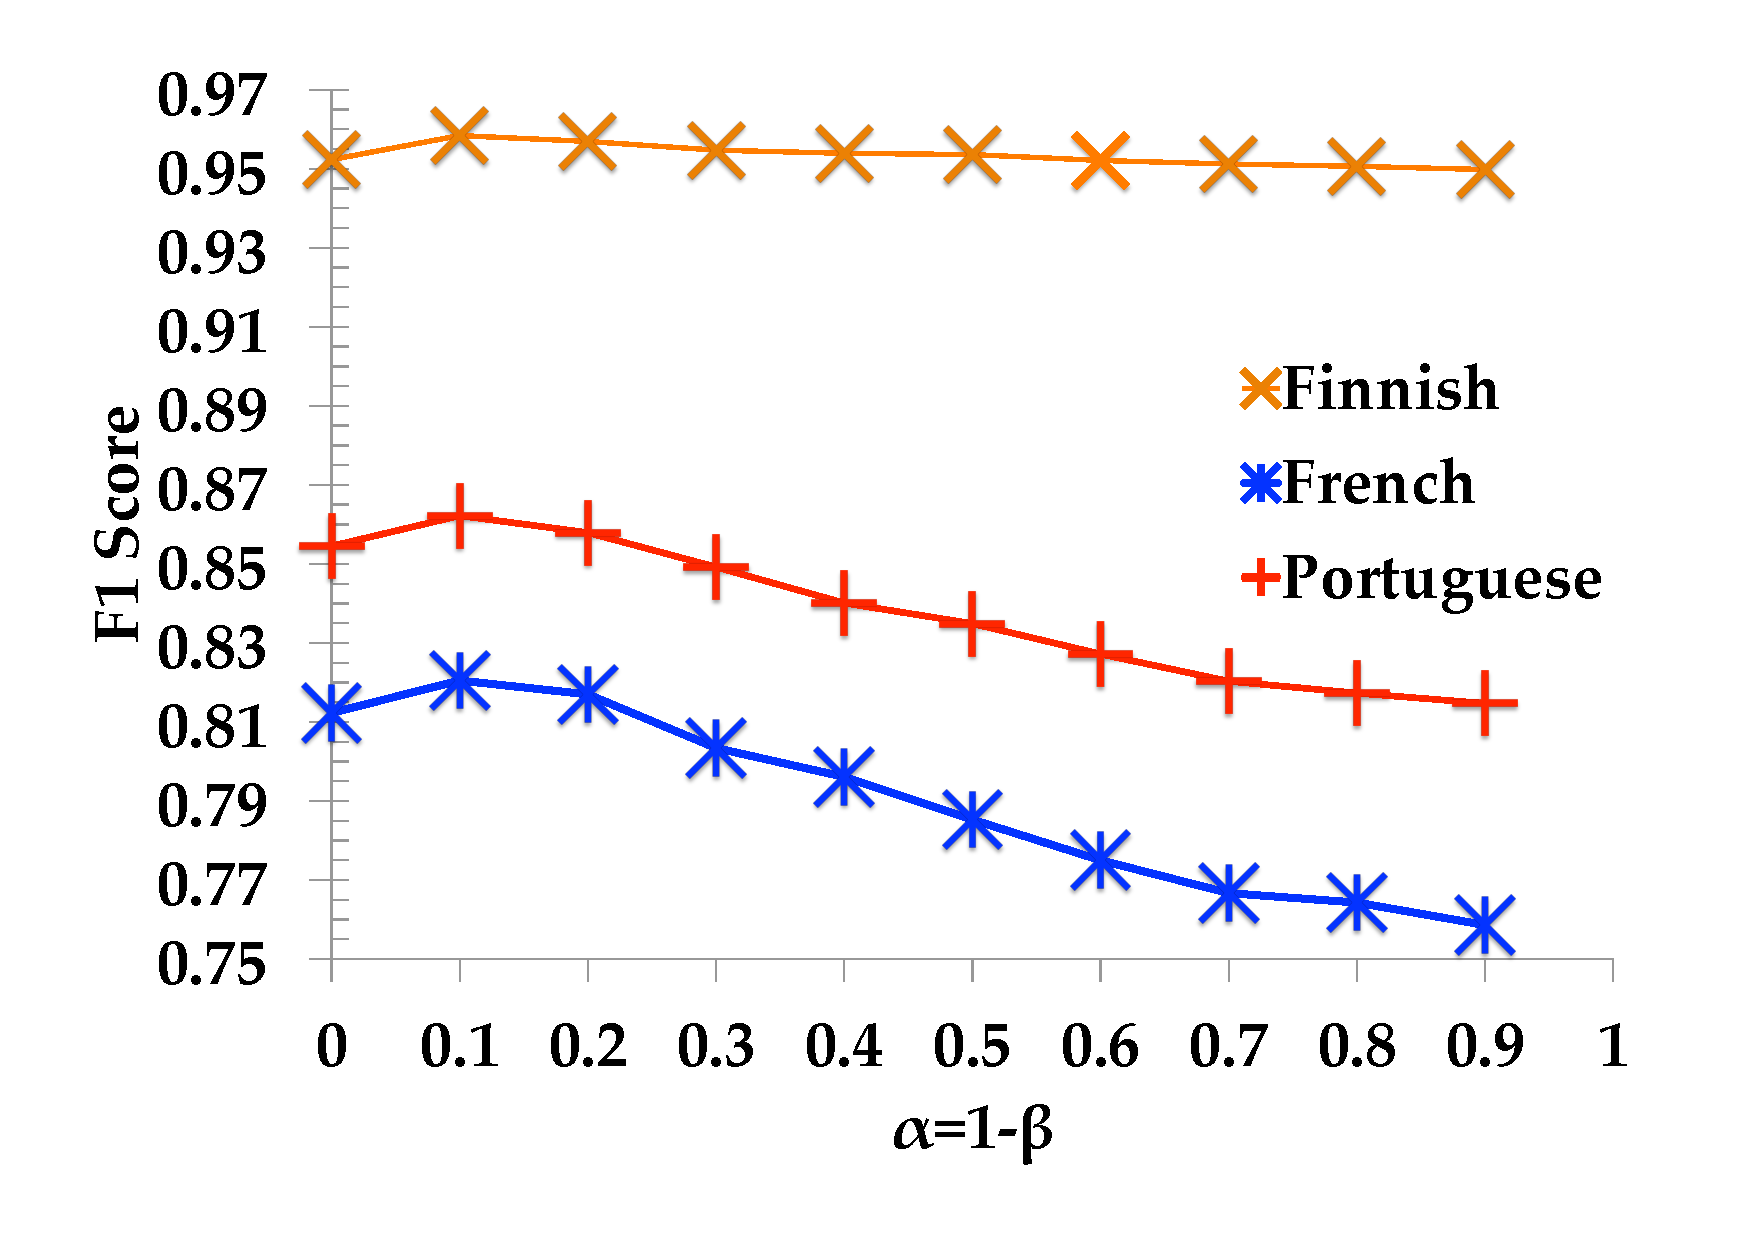
\includegraphics[width=0.64\columnwidth]{alphabetafig}
\caption{F1 score for Finnish, French and Portuguese depending on the value of \(\alpha\) and \(\beta\).}
\label{fig.1}
\end{figure}

\subsubsection{Optimal \(\delta\) selection}
Now that we have fixed the best values of \(\alpha\) and \(\beta\), we can search for the best value for \(\delta\). We make delta vary in steps of \(0.05\) between \(0\) and \(0.3\). The choice of the upper bound is based on the hypothesis that the optimal value is somewhere closer to 0, as a too large threshold essentially means that that most or all senses will be considered as disambiguation of the translation, as if, we had disambiguated nothing. 

The \(\delta\) heuristic affects the results of the disambiguation whether the measure is  Tversky index or another Level 2 Textual similarity. Thus, in this experiment, we will also include Level 2 version of the three string distance measures that we used in the first experiment.

Figure \ref{fig.2} graphically presents the \(F1\) scores for each value of \(delta\) and each language. The first apparent trend is that Level 2 measures systemically perform much worse (by up to 30\%) than our own similarity measure. Depending on the language different values of \(delta\) are optimal, even though it is difficult to see a great difference. For French \(\delta=0.10\), for Finnish \(\delta=0.15\)
 and for Portuguese \(\delta=0.10\). 
In all three previous experiments, it became apparent, that the same string similarity measure, the same values for alpha and beta as well as the same value for delta were optimal, which leads us to believe that their optimality will be conserved across all languages. However, especially for the string similarity measure, it is reasonable to believe that for languages such a Chinese or Japanese that lack segmentation, the optimal choice for the string distance measure may be entirely different.
\subsection{Final Disambigation Results}

Now that we estimated the optimal parameters, we can present the final results based on them in Table \ref{tab:final}). We use the chance of random selection as well as the most frequent sense selection as baselines for this comparison.

The first thing one can notice is that there is a stark difference between the scores of Finnish, and the rest. Indeed, first of all, the random baseline and most frequent sense baselines are an indication that the French and Portuguese DBNaries are highly polysemous, while Finnish contains a very large amount of monosemous entries, which artificially inflates the value of the score. 

Interestingly he random baseline is higher (up to 6.6\%) than the most frequent sense baseline, which indicates that the first sense if often not the right sense to select to match the translation. This could be explained by the fact that translations in other language can often lead to different target words for every source sense and thus selecting the first sense will be correct of a most a small proportion of the translation relations leaving from the source word.

We can see that for all three languages we achieve a good performance compared to what is presented in the literature, most notably in the fact that most of the errors, can easily be identified as such just by looking at whether they produced any overlap.

\begin{table}
{\centering \footnotesize
\begin{tabular}{|c|c|c|c|c|c|}
\hline &P&R&F1&MFS F1&Random\\
\hline Portuguese&0.8572&0.8814&0.8651&0.2397&0.3103\\
\hline Finnish&0.9642&0.9777&0.9687&0.7218&0.7962\\
\hline French&0.8267&0.8313&0.8263&0.3542&0.3767\\
\hline 
\end{tabular}
\caption{Final results with optimal measure and parameter values. Precision, Recall, F1 score for all three languages compared against the MFS and Random Baselines.}
\label{tab:final}
}
\end{table} 

\begin{figure}
\centering
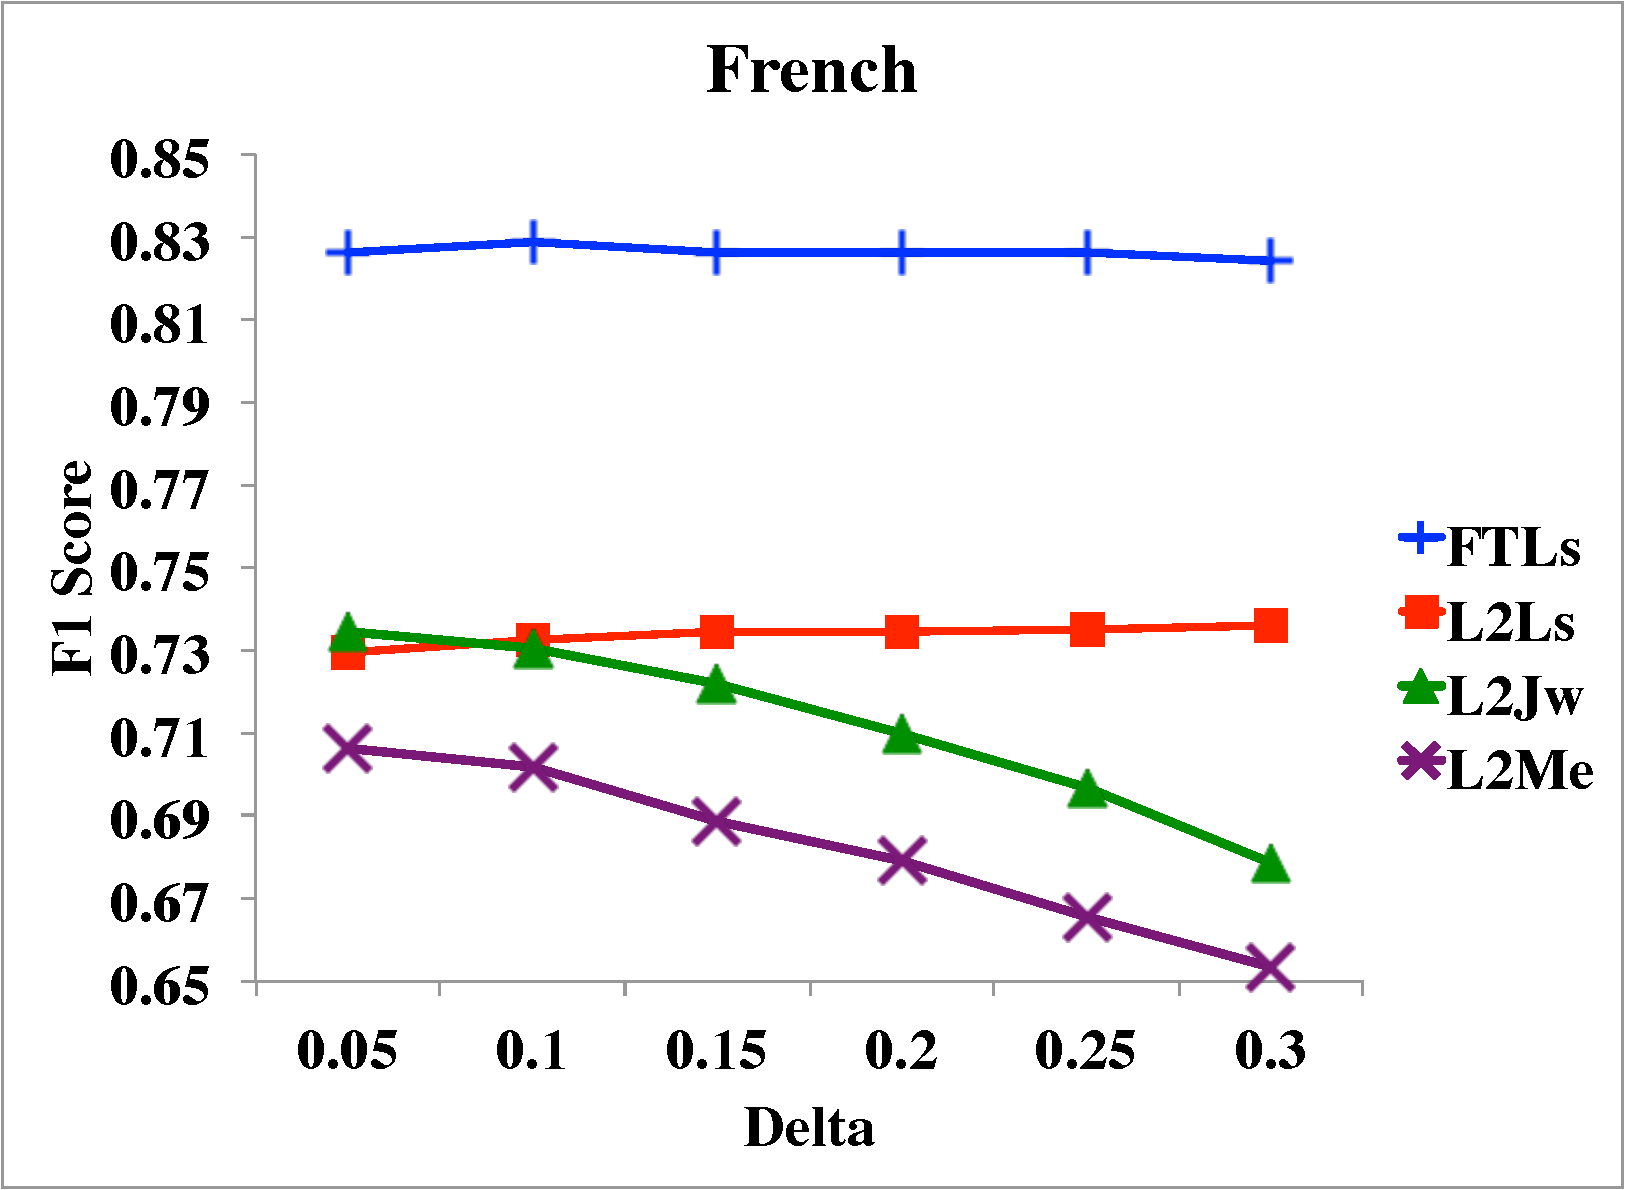
\includegraphics[width=.55\columnwidth]{french}
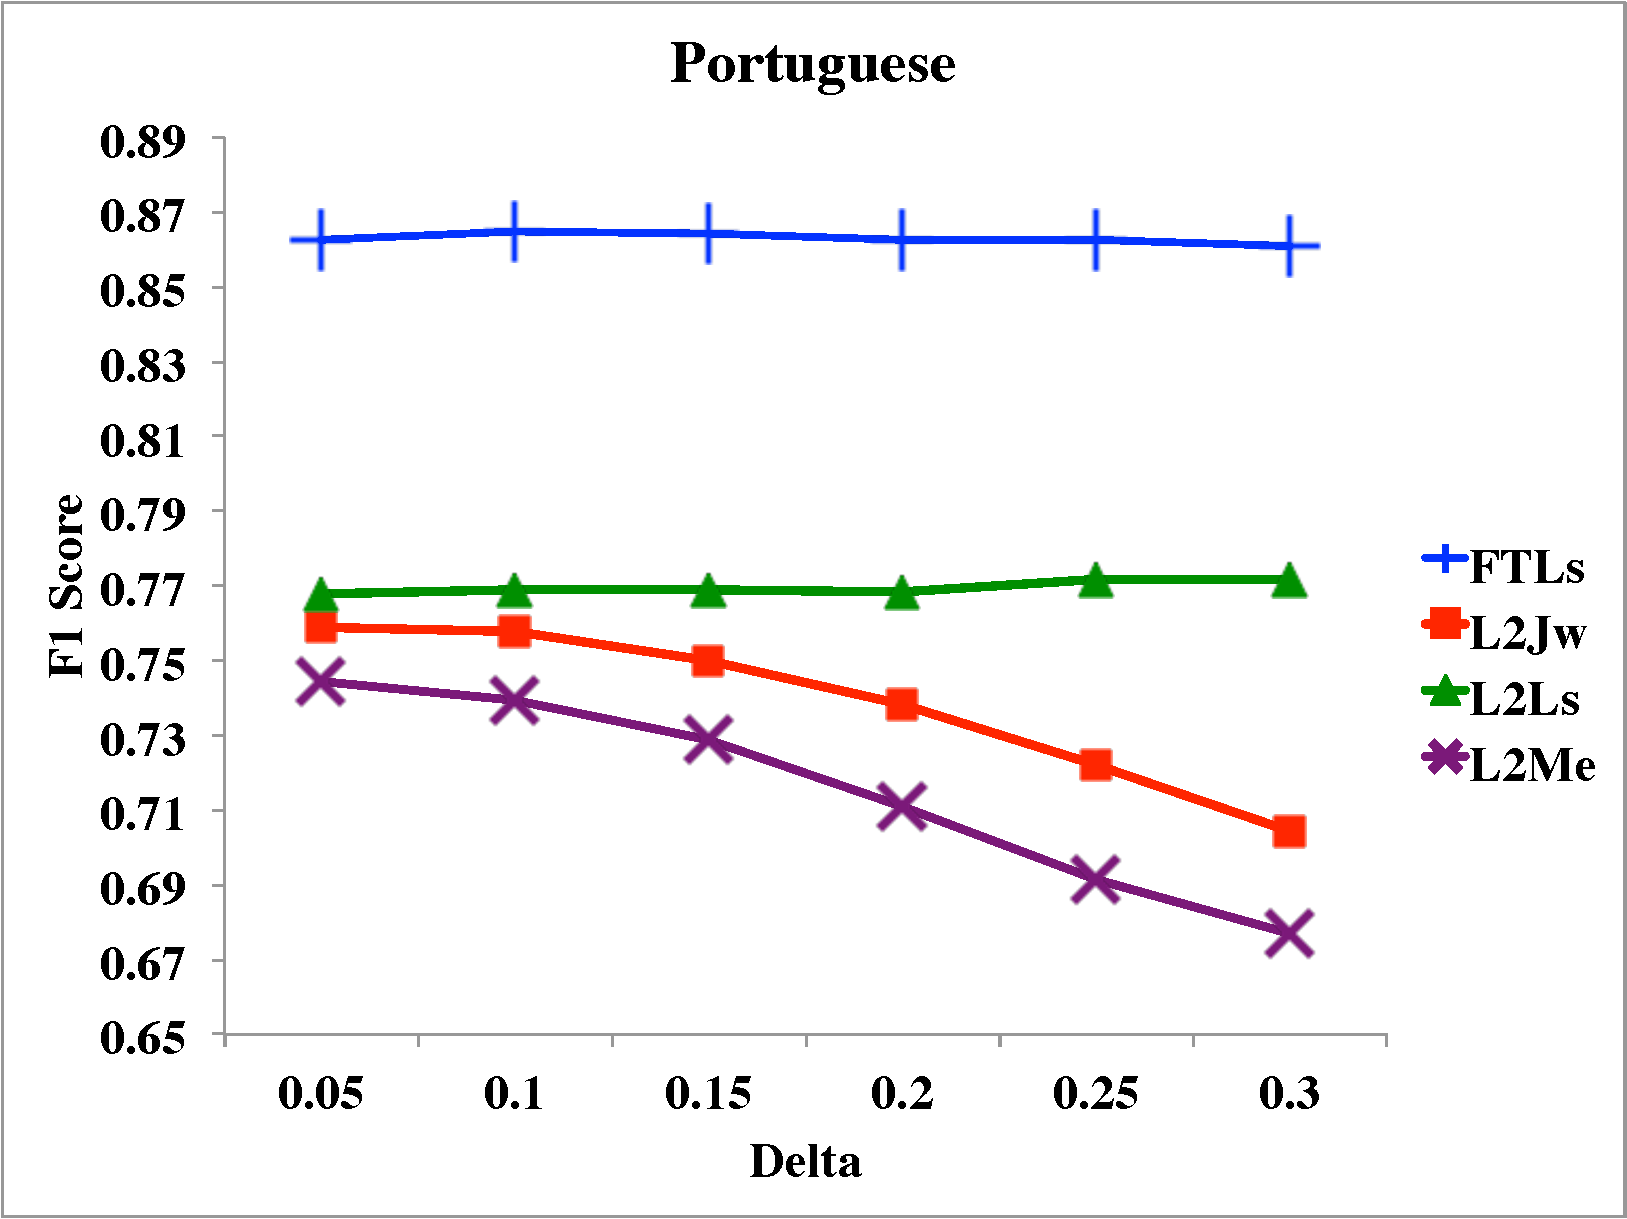
\includegraphics[width=.55\columnwidth]{portuguese}
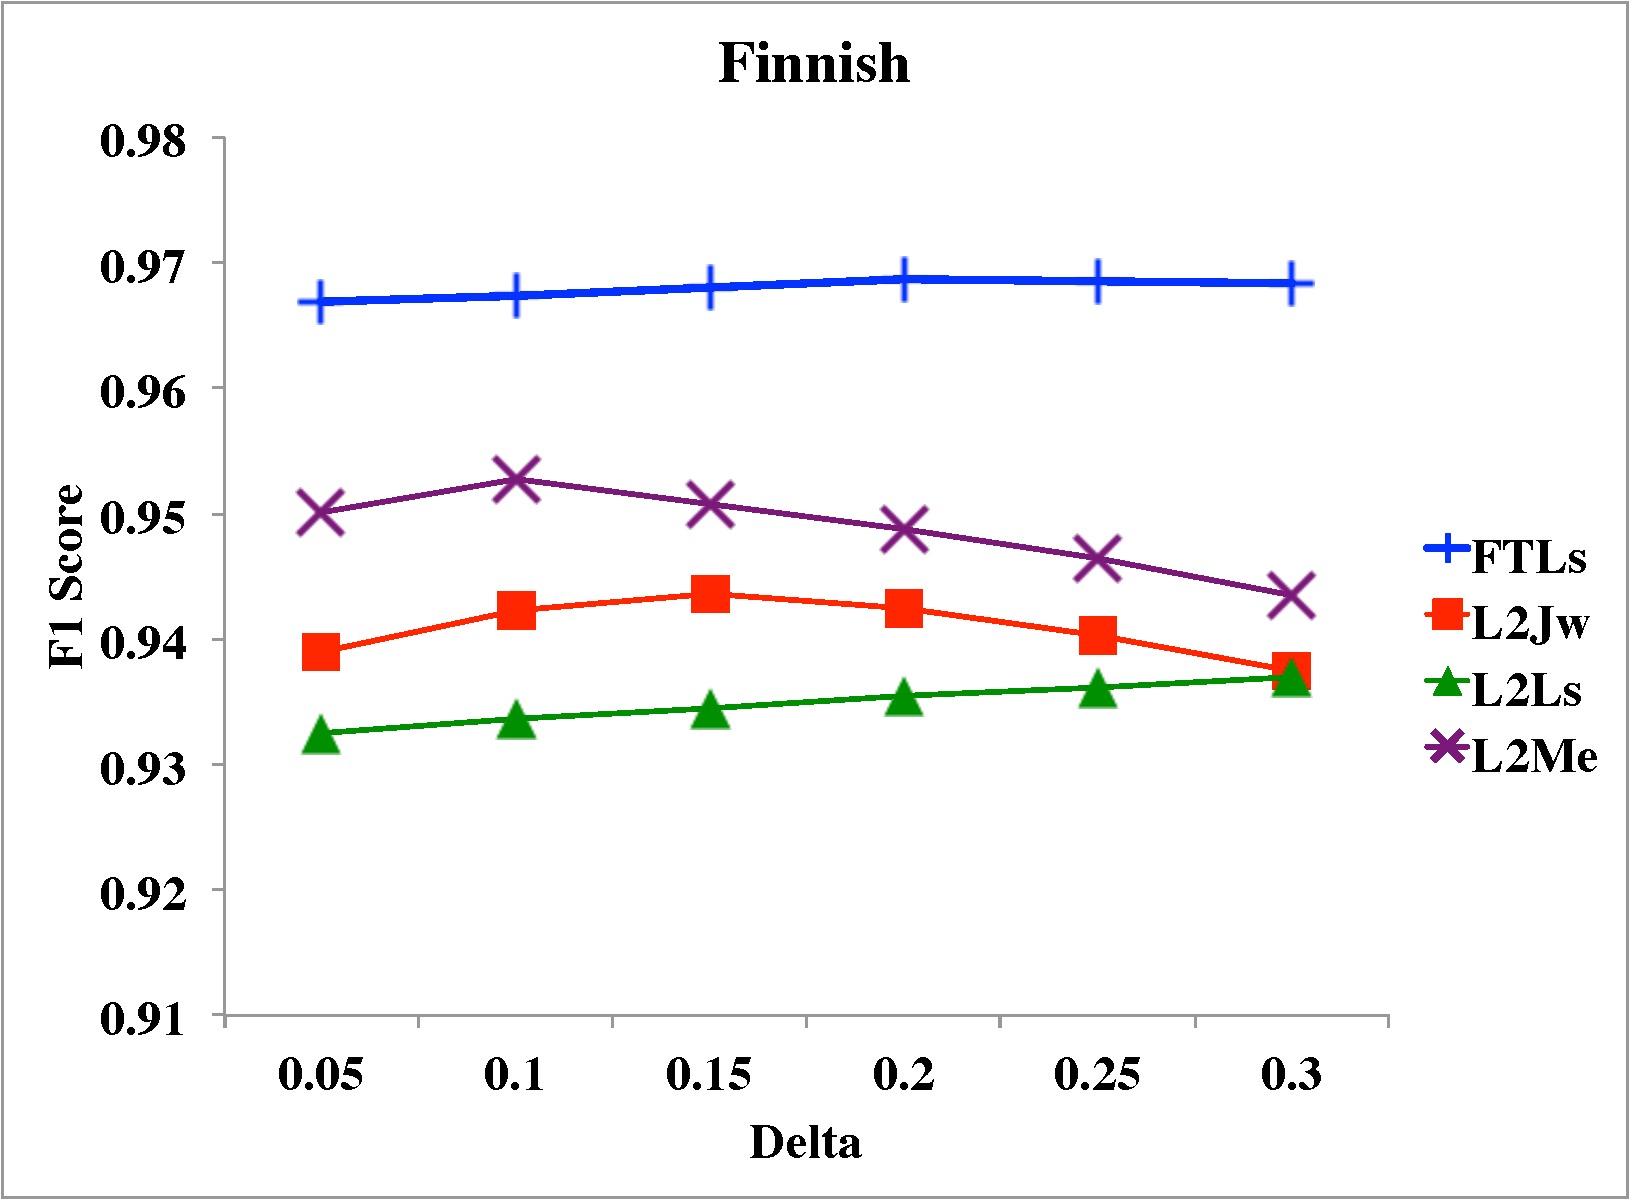
\includegraphics[width=.55\columnwidth]{finnish}
\caption{Graphical representation of the F1 score against delta for our measure and other Level 2 Measures.}
\label{fig.2}
\end{figure}

\subsection{Error analysis}

We did not perform a full fledged and systematic error analysis, but rather an informal manual sampling so as to have an idea of what the error can be and if there are ways to correct them by adapting the measures or the methodology.
We looked at some of the errors and manually categorized them: 
\begin{enumerate}
\item No overlap between the gloss and sense definitions (Random choice by our algorithm), this happens when the translation gloss is a paraphrase of the sense definition or simply a metaphor for it.
\item The overlap is with the domain category label or the example glosses, which we do not currently extract. This is a particular case of the first type of error.
\item New senses have been introduced in Wiktionary and shifted sense numbers, which were not subsequently updated in the resource. Such errors cannot be detected during the extraction process.
\end{enumerate}

We can in fact easily find all the errors due to the lack of overlap and correct the errors of type 2 by enriching the extraction process of DBnary. Thus we can single-out errors that are due to inconsistencies in the resource and thus potentially use the disambiguation results to indicate to users where errors are located an need to be updated.

\section{Conclusion}

With our method, we were able to find an optimal similarity measure for translation disambiguation in DBnary. Similar results across three languages suggests that it is a general optimality that can be applied to all the languages currently present in DBnary, although for Asian Languages that have no segmentation, it is likely not the case.

Then, we compared the results and concluded that our method is viable for the task of disambiguating glossed translation relations, especially considering the low random baselines and first sense baselines compared to the top score of our method.

For translation relations without glosses, the disambiguation process is more complex and is part of the Future Work that we plan on carrying out.

\section{Acknowledgements}

This work was conducted as a part of the CHIST-ERA CAMOMILE project,
which was funded by the ANR (Agence Nationale de la Recherche, France).
%\nocite{*}

\bibliographystyle{lrec2006}
\bibliography{dbnary-wsd}

\end{document}

\begin{figure}[h]
\begin{center}
%\fbox{\parbox{6cm}{
%This is a figure with a caption.}}
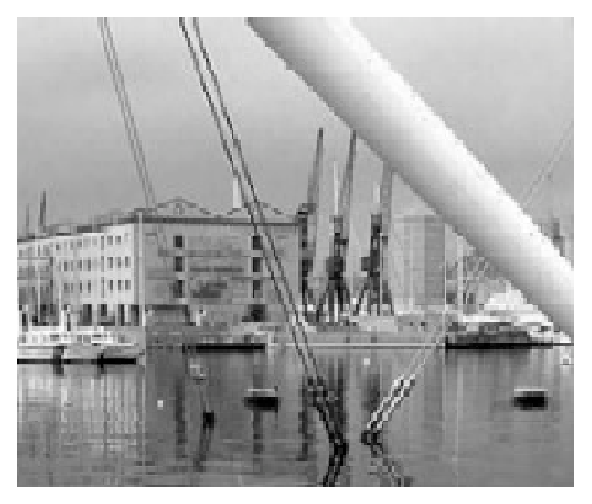
\includegraphics[scale=0.5]{image1.eps} 
\caption{The caption of the figure.}
\label{fig.1}
\end{center}
\end{figure}

\section{Footnotes}

Footnotes are indicated within the text by a number in superscript\footnote{They should be in Times 9, and appear at the bottom of the same page as their corresponding number. Footnotes should also be separated from the rest of the text by a horizontal line 5 cm long.}.

\section{Copyrights}

The Lan\-gua\-ge Re\-sour\-ce and Evalua\-tion Con\-fe\-rence (LREC) proceedings are published by the European Language Resources Association (ELRA). They include different media that may be used (i.e. hardcopy, CD-ROM, Internet-based/Web, etc.).

ELRA's policy is to acquire copyright for all LREC contributions. In assigning your copyright, you are not forfeiting your right to use your contribution elsewhere. This you may do without seeking permission and is subject only to normal acknowledgement to the LREC proceedings.
